
\documentclass{beamer}

\usepackage{cmap}				% To be able to copy-paste russian text from pdf
\usepackage[T2A]{fontenc}
\usepackage[utf8]{inputenc}
\usepackage[english]{babel}
\usepackage{textpos}
\usepackage{ragged2e}
\usepackage{amssymb}
\usepackage{ulem}
\usepackage{tikz}
\usepackage{pgfplots}
\usepackage{color}
\usepackage{cancel}
\usepackage{multirow}
\pgfplotsset{compat=1.17}
\usetikzlibrary{arrows,snakes,backgrounds,shapes}
\usepgfplotslibrary{groupplots,colorbrewer,dateplot,statistics}
\usepackage{animate}

\usepackage{amsfonts}
\usepackage{amsmath}
\usepackage{amssymb}
\usepackage{graphicx}
\usepackage{setspace}
\usepackage{cancel}

\usepackage{enumitem}
\setitemize{label=\usebeamerfont*{itemize item}%
  \usebeamercolor[fg]{itemize item}
  \usebeamertemplate{itemize item}}

% remove navigation bar
\setbeamertemplate{navigation symbols}{} 

\usepackage{eurosym}
\renewcommand{\EUR}[1]{\textup{\euro}#1}

\title{Black-Scholes Model}
\author{Artem Bakulin}
\date{November 5, 2024}

\usetheme{Warsaw}
\usecolortheme{beaver}

\setbeamertemplate{page number in head/foot}[totalframenumber] 

\newcommand{\ru}[1]{\begin{otherlanguage}{russian}#1\end{otherlanguage}}
\newcommand{\en}[1]{\begin{otherlanguage}{english}#1\end{otherlanguage}}
\newcommand{\ruen}[2]{#1 (\en{#2})}

\begin{document}



\begin{frame}
\titlepage
\end{frame}


\newcommand{\drawStockNode}[5]{

	\node (#5)
	[
		draw,
		rectangle,
		rounded corners,
		inner sep = 0pt,
		outer sep = 0pt,
		minimum width = 2.4cm,
		minimum height = 0.55cm,
		align = center
	]
	at (#3, #4)
	{
		\begin{tabular}{c|c}
		#1 & #2
		\end{tabular}
	};
}

\newcommand{\drawStockLink}[4]{

	\draw[
		->,
		>=triangle 90
	]
	(#1.east) -- (#2.west)
	node[
		pos = 0.5,
		anchor = #4
	]
	{#3};
}

\newcommand{\drawOneStepBinomialTree}{
	\drawStockNode{\$100}{?}{0}{0}{S0_node}
	\drawStockNode{\$120}{\$20}{4}{ 1}{Su_node}
	\drawStockNode{\$80}{\$0}{4}{-1}{Sd_node}
	
	\drawStockLink{S0_node}{Su_node}{$90\%$}{south east}	
	\drawStockLink{S0_node}{Sd_node}{$10\%$}{north east}
}



\renewcommand{\drawOneStepBinomialTree}{
	\drawStockNode{$S_0$}{?}{0}{0}{S0_node}
	\drawStockNode{$S_0u$}{$V_u$}{4}{ 1}{Su_node}
	\drawStockNode{$S_0d$}{$V_d$}{4}{-1}{Sd_node}
	
	\drawStockLink{S0_node}{Su_node}{$p$}{south east}	
	\drawStockLink{S0_node}{Sd_node}{$1 - p$}{north east}
}

\begin{frame}{Recap: binomial model}
\centering
\begin{tikzpicture}
	\drawOneStepBinomialTree
\end{tikzpicture}

\justify
Current stock price is $S_0$.

\justify
Stock price can either increase to $S_0\cdot u$ (u>1) or drop to $S_0 \cdot d$ (d<1).

\justify
Single period of $\tau$ years, risk-free interest rate is $r$, such that $d < 1+r\tau < u$.

\justify
A derivative pays off (has the value of) either $V_u$ or $V_d$ depending on the stock price moving up or down.

\end{frame}



\begin{frame}{Recap: binomial model - 2}
\centering
\begin{tikzpicture}
	\drawOneStepBinomialTree
\end{tikzpicture}

\justify
Consider a portfolio of $\Delta$ stock and debt $L$. 
\begin{equation*}
\begin{cases}
L(1+r\tau) + \Delta S_0 u = V_u \\
L(1+r\tau) + \Delta S_0 d = V_d
\end{cases}
\end{equation*}

\begin{equation*}
\begin{cases}
\Delta = \dfrac{V_u - V_d}{S_0(u-d)} \\
L = \dfrac{V_du - V_ud}{(1+r\tau)(u-d)}
\end{cases}
\end{equation*}
\end{frame}



\begin{frame}{Recap: binomial model - 3}
\centering
\begin{tikzpicture}
\drawOneStepBinomialTree
\end{tikzpicture}

\justify
The option is worth the same as the replicating portfolio:
\begin{align*}
C &= \Delta S_0 +L = \\
 &= \dfrac{V_u-V_d}{(u-d)\cancel{S_0}}\cancel{S_0} + \dfrac{V_du -V_ud}{(1+r\tau)(u-d)} = \\
 &= \dfrac{qV_u +(1-q)V_d}{1+r\tau},
\end{align*}
where
\begin{equation*}
q = \dfrac{1+r\tau - d}{u-d}
\end{equation*}
This magic parameter $q$ is called the "risk-neutral probability".
\end{frame}



\renewcommand{\drawStockLink}[2]{

	\draw[
		->,
		>=triangle 45
	]
	(#1.east) -- (#2.west)
	{};
}

\renewcommand{\drawStockNode}[5]{

	\node (#5)
	[
		draw,
		rectangle,
		rounded corners,
		inner sep = 1pt,
		outer sep = 0pt,
		minimum width = 1.5cm
	]
	at (#3, #4)
	{
		\centering
		\begin{tabular}{c}
		#1 \\ \hline #2
		\end{tabular}
	};
}

\newcommand{\nodeVerticalStep}{0.7}
\newcommand{\nodeHorizontalStep}{2.75}

\begin{frame}{Recap: binomial model - 4}
\centering
\begin{tikzpicture}
\drawStockNode{$\$100$}{\only<1-7>{?}\only<8->{\$14.8}}{0}{0}{S0_node}

\drawStockNode{$\$120$}{\only<1-5>{?}\only<6->{\$25.8}}{\nodeHorizontalStep}{\nodeVerticalStep}{Su_node}
\drawStockNode{$\$80$}{\only<1-6>{?}\only<7->{\$3.8}}{\nodeHorizontalStep}{-\nodeVerticalStep}{Sd_node}

\drawStockNode{$\$144$}{\only<1-2>{?}\only<3->{\$44}}{2*\nodeHorizontalStep}{2*\nodeVerticalStep}{Suu_node}
\drawStockNode{$\$96$}{\only<1-3>{?}\only<4->{\$7.6}}{2*\nodeHorizontalStep}{0}{Sud_node}
\drawStockNode{$\$64$}{\only<1-4>{?}\only<5->{\$0}}{2*\nodeHorizontalStep}{-2*\nodeVerticalStep}{Sdd_node}

\drawStockNode{$\$172.8$}{\only<1>{?}\only<2->{\$72.8}}{3*\nodeHorizontalStep}{3*\nodeVerticalStep}{Suuu_node}
\drawStockNode{$\$115.2$}{\only<1>{?}\only<2->{\$15.2}}{3*\nodeHorizontalStep}{\nodeVerticalStep}{Suud_node}
\drawStockNode{$\$76.8$}{\only<1>{?}\only<2->{\$0}}{3*\nodeHorizontalStep}{-\nodeVerticalStep}{Sudd_node}
\drawStockNode{$\$51.2$}{\only<1>{?}\only<2->{\$0}}{3*\nodeHorizontalStep}{-3*\nodeVerticalStep}{Sddd_node}

\drawStockLink{S0_node}{Su_node}
\drawStockLink{S0_node}{Sd_node}

\drawStockLink{Su_node}{Suu_node}
\drawStockLink{Su_node}{Sud_node}

\drawStockLink{Sd_node}{Sud_node}
\drawStockLink{Sd_node}{Sdd_node}

\drawStockLink{Suu_node}{Suuu_node}
\drawStockLink{Suu_node}{Suud_node}

\drawStockLink{Sud_node}{Suud_node}
\drawStockLink{Sud_node}{Sudd_node}

\drawStockLink{Sdd_node}{Sudd_node}
\drawStockLink{Sdd_node}{Sddd_node}
\end{tikzpicture}

\justify
Suppose that $u=1.2$, $d=0.8$, $S_0=\$100$, $r=0\%$. What is fair value of a call option at strike $K=100$?

\justify
The "risk-neutral probability":
\begin{align*}
q = \dfrac{1+r\tau - d}{u - d} = \dfrac{1 - 0.8}{1.2 - 0.8} = 0.5
\end{align*}
\end{frame}



\begin{frame}{Recap: binomial model - 5}
\centering
\begin{tikzpicture}
\drawStockNode{$\$100$}{$\Delta=0.55$}{0}{0}{S0_node}

\drawStockNode{$\$120$}{$\Delta=0.76$}{\nodeHorizontalStep}{\nodeVerticalStep}{Su_node}
\drawStockNode{$\$80$}{$\Delta=0.24$}{\nodeHorizontalStep}{-\nodeVerticalStep}{Sd_node}

\drawStockNode{$\$144$}{$\Delta=1.0$}{2*\nodeHorizontalStep}{2*\nodeVerticalStep}{Suu_node}
\drawStockNode{$\$96$}{$\Delta=0.4$}{2*\nodeHorizontalStep}{0}{Sud_node}
\drawStockNode{$\$64$}{$\Delta=0.0$}{2*\nodeHorizontalStep}{-2*\nodeVerticalStep}{Sdd_node}

\drawStockNode{$\$172.8$}{$\Delta=1$}{3*\nodeHorizontalStep}{3*\nodeVerticalStep}{Suuu_node}
\drawStockNode{$\$115.2$}{$\Delta=1$}{3*\nodeHorizontalStep}{\nodeVerticalStep}{Suud_node}
\drawStockNode{$\$76.8$}{$\Delta=0$}{3*\nodeHorizontalStep}{-\nodeVerticalStep}{Sudd_node}
\drawStockNode{$\$51.2$}{$\Delta=0$}{3*\nodeHorizontalStep}{-3*\nodeVerticalStep}{Sddd_node}

\drawStockLink{S0_node}{Su_node}
\drawStockLink{S0_node}{Sd_node}

\drawStockLink{Su_node}{Suu_node}
\drawStockLink{Su_node}{Sud_node}

\drawStockLink{Sd_node}{Sud_node}
\drawStockLink{Sd_node}{Sdd_node}

\drawStockLink{Suu_node}{Suuu_node}
\drawStockLink{Suu_node}{Suud_node}

\drawStockLink{Sud_node}{Suud_node}
\drawStockLink{Sud_node}{Sudd_node}

\drawStockLink{Sdd_node}{Sudd_node}
\drawStockLink{Sdd_node}{Sddd_node}
\end{tikzpicture}

\justify
Fair arbitrage-free value of an option does not depend on the probability of the stock price changing up or down. We can replicate any option by \alert{dynamically} re-balancing the replicating portfolio (a stock and debt) at each node.

\justify
This strategy is also called the \alert{delta hedging}.
\end{frame}



\newcommand{\highlightStockLink}[6]{
	\draw[
		color=#4,
		very thick,
		->,
		>=triangle 45
	]
	(#1.east) -- (#2.west)
	node[
		pos=#5,
		anchor=#6
	]
	{#3};
}

\newcommand{\highlightStockLinkUp}[3]{
	\highlightStockLink{#1}{#2}{$q$}{#3}{0.5}{south}
}

\newcommand{\highlightStockLinkDown}[3]{
	\highlightStockLink{#1}{#2}{$1-q$}{#3}{0.15}{west}
}

\begin{frame}{Recap: risk-neutral probability}
\centering
\begin{tikzpicture}
\drawStockNode{$S_0$}{?}{0}{0}{S0_node}

\drawStockNode{$S_0u$}{?}{\nodeHorizontalStep}{\nodeVerticalStep}{Su_node}
\drawStockNode{$S_0d$}{?}{\nodeHorizontalStep}{-\nodeVerticalStep}{Sd_node}

\drawStockNode{$S_0u^2$}{?}{2*\nodeHorizontalStep}{2*\nodeVerticalStep}{Suu_node}
\drawStockNode{$S_0ud$}{?}{2*\nodeHorizontalStep}{0}{Sud_node}
\drawStockNode{$S_0d^2$}{?}{2*\nodeHorizontalStep}{-2*\nodeVerticalStep}{Sdd_node}

\drawStockNode{$S_0u^3$}{$V_3$}{3*\nodeHorizontalStep}{3*\nodeVerticalStep}{Suuu_node}
\drawStockNode{$S_0u^2d$}{$V_2$}{3*\nodeHorizontalStep}{\nodeVerticalStep}{Suud_node}
\drawStockNode{$S_0ud^2$}{$V_1$}{3*\nodeHorizontalStep}{-\nodeVerticalStep}{Sudd_node}
\drawStockNode{$S_0d^3$}{$V_0$}{3*\nodeHorizontalStep}{-3*\nodeVerticalStep}{Sddd_node}

\only<1-2>{
	\drawStockLink{S0_node}{Su_node}
	\drawStockLink{S0_node}{Sd_node}

	\drawStockLink{Su_node}{Suu_node}
	\drawStockLink{Su_node}{Sud_node}

	\drawStockLink{Sd_node}{Sud_node}
	\drawStockLink{Sd_node}{Sdd_node}

	\drawStockLink{Suu_node}{Suuu_node}
	\drawStockLink{Suu_node}{Suud_node}

	\drawStockLink{Sud_node}{Suud_node}
	\drawStockLink{Sud_node}{Sudd_node}

	\drawStockLink{Sdd_node}{Sudd_node}
	\drawStockLink{Sdd_node}{Sddd_node}
}

\only<3>{
	\highlightStockLinkUp{S0_node}{Su_node}{Set1-A}
	\highlightStockLinkUp{Su_node}{Suu_node}{Set1-A}
	\highlightStockLinkDown{Suu_node}{Suud_node}{Set1-A}
}

\only<4>{
	\highlightStockLinkUp{S0_node}{Su_node}{Set1-A}
	\highlightStockLinkDown{Su_node}{Sud_node}{Set1-A}
	\highlightStockLinkUp{Sud_node}{Suud_node}{Set1-A}
}

\only<5>{
	\highlightStockLinkDown{S0_node}{Sd_node}{Set1-A}
	\highlightStockLinkUp{Sd_node}{Sud_node}{Set1-A}
	\highlightStockLinkUp{Sud_node}{Suud_node}{Set1-A}
}

\end{tikzpicture}

\justify
Risk-neutral probability: $q = \dfrac{1 + rT - d}{u - d}$.

\justify
Fair value of an option today:
\begin{align*}
V = \frac{q^3V_3 + \only<1>{3q^2(1-q)}\only<2->{\alert{3q^2(1-q)}}V_2 + 3q(1-q)^2V_1 + (1-q)^3V_0}{(1+rT)^3}
\end{align*}
\end{frame}



\begin{frame}{Recap: risk-neutral probability - 2}
\justify
Close your eyes and pretend that $q$ is the probability of the sock price moving up (in reality it is not). Then $3q^2(1-q)$ is probability of the stock moving up twice and moving down once. In this scenario the stock is worth  $S_0u^2d$, and the option pays off $V_2$.

\justify
\centering
\begin{tabular}{l|l|l}
Stock price & Payoff & "Probability" \\ \hline
$S_0u^3$   & $V_3$   & $q^3$ \\
$S_0u^2d$  & $V_2$   & $3q^2(1-q)$ \\
$S_0ud^2$  & $V_1$   & $3q(1-q)^2$ \\ 
$S_0d^3$   & $V_0$   & $(1-q)^3$ 
\end{tabular}

\justify
Fair value of an option looks similar to the discounted "expected"\ payoff.
\begin{align*}
V = \frac{q^3V_3 + 3q^2(1-q)V_2 + 3q(1-q)^2V_1 + (1-q)^3V_0}{(1+rT)^3}
\end{align*}
\end{frame}



\begin{frame}{Binomial model and the Black-Scholes model}
Consider a binomial tree that consists of $n$ steps:
\begin{align*}
C &= \dfrac{\sum\limits_{k=0}^{n} C^k_nq^k(1-q)^{n-k}V(S_0u^kd^{n-k})}{(1+r\tau)^n} \\
C^k_n &= \dfrac{n!}{k!(n-k)!}
\end{align*}

\justify
What if we replace the function $V(S)$ with the call option payoff $max(S-K,0)$, and let $n$ tend towards infinity? We will get the famous Black-Scholes formula!

\justify
Please have a look at rigorous proof here (28 pages):

\url{http://www.math.cmu.edu/~handron/21_370/BS.pdf}
\end{frame}



\begin{frame}{Demo: Galton board}

\url{https://www.mathsisfun.com/data/quincunx.html}
\end{frame}



\begin{frame}{Central limit theorem}
\justify
Suppose that $\xi_i$ are independent identically distributed (i.i.d.) random variables, with finite expected value $\mathbb{E}\xi_i=\mu$ and finite variance $\operatorname{Var}(\xi_i) = \sigma^2$. Then there is a convergence by distribution:
\begin{align*}
\lim_{n \to \infty} \sqrt{n}\frac{\dfrac{1}{n}\sum\limits_{i=1}^{n}\xi_i - \mu}{\sigma} = \mathcal{N}(0, 1)
\end{align*}

\justify
Here $\mathcal{N}(0, 1)$ is standard normal (Gaussian) distribution.

\justify
This is the Central Limit Theorem (CLT). Arithmetic mean of a large sample of i.i.d. variables tends to normal distribution.
\end{frame}




\begin{frame}{Geometric deterministic motion}
\justify
Consider an option that expires in $T$ years. Lets split this interval into $N$ equal time steps, so that each sub-interval has duration of $dt = T/N$ years.

\justify
Suppose that there is no randomness. At each time step $dt$ the stock price grows by $\mu$ percent per annum (simple interest rate without compounding). 
\begin{align*}
\frac{S_{i+1} - S_i}{S_i} = \mu dt \quad \Rightarrow \quad S_{i+1} = S_i(1 + \mu dt)
\end{align*}

\justify
What will be the stock price in $T$ years after $N$ steps, if each step is $dt=T/N$ years?
\begin{align*}
S_T &= S_N = S_{N-1}\left(1+\mu\dfrac{T}{N}\right) 
= S_{N-2}\left(1+\mu\dfrac{T}{N}\right)\left(1+\mu\dfrac{T}{N}\right) = \\
&= S_0\left(1+\mu\dfrac{T}{N}\right)^N \to S_0e^{\mu T}
\end{align*}

\justify
This is a familiar formula for continuously compounded interest rate.
\end{frame}



\newcommand{\plotDterministicMotion}[2] {
	
	\addplot[
		color = #2,
		mark = none,
		thick
	] 
	table[
		x=t,
		y=trend,
		col sep=comma
	]
	{#1};
}



\begin{frame}{Geometric deterministic motion: an example}
\centering
\begin{tikzpicture}
\begin{axis}[
  width=\textwidth,
  height=\textheight - 1cm,
  xlabel near ticks,
  ylabel near ticks,
  xmin=0, xmax=1,
  ymin=75,ymax=125,
  legend entries = {
  	   {$\mu=5\%$},
     	  {$\mu=10\%$}
  },
  legend cell align={left},
  legend style={at={(0.97,0.03)},anchor=south east}
]

	\plotDterministicMotion{gbm_sample_100.csv}{Set1-A}
	\plotDterministicMotion{gbm_sample_500.csv}{Set1-B}
\end{axis}
\end{tikzpicture}
\end{frame}



\begin{frame}{Geometric Brownian motion}
\justify
Let the stock price randomly fluctuate  around the deterministic trend $\mu$ at each step.

\justify
How do we define randomness? Suppose that the fluctuations reflect incoming bits of information ("shocks"), and that these shocks are independent. Then we can hope that these shocks add up to a normal distribution.
 \begin{align*}
\frac{S_{i+1} - S_i}{S_i} = \mu dt + \sigma\xi_i\sqrt{dt}, \quad \xi_i \sim \mathcal{N}(0, 1)
\end{align*}

Here $\xi_i$ are random shocks that pull the stock price up and down, $\sigma$ is volatility or standard deviation. Usually we measure the volatility $\sigma$ in percent per annum, just like interest rates or the trend $\mu$.

\justify
This is Geometric Brownian Motion (GBM). GBM is the limit of a binomial tree if we define $u$ and $d$ as follows:
\begin{align*}
u &= e^{\mu dt + \sigma\sqrt{dt}} \\
d &= e^{\mu dt - \sigma\sqrt{dt}}
\end{align*}
\end{frame}



\newcommand{\plotBrownianMotion}[2] {
	
	\addplot[
		color = #2,
		mark = none,
		thick
	]
	table[
		x=t,
		y=s,
		col sep=comma
	]
	{#1};
	
	\addplot[
		color = #2,
		mark = none,
		thick,
		dashed,
		forget plot
	] 
	table[
		x=t,
		y=trend,
		col sep=comma
	]
	{#1};
}

\begin{frame}{Geometric Brownian Motion: an example}
\centering
\begin{tikzpicture}
\begin{axis}[
  width=\textwidth,
  height=\textheight - 1cm,
  xlabel near ticks,
  ylabel near ticks,
  xmin=0, xmax=1,
  ymin=75,ymax=125,
  legend entries = {
  	   {$\mu=5\%, \sigma=10\%, N=100$},
      {$\mu=10\%, \sigma=40\%, N=500$}
  },
  legend cell align={left},
  legend style={at={(0.97,0.03)},anchor=south east}
]

	\plotBrownianMotion{gbm_sample_100.csv}{Set1-A}
	\plotBrownianMotion{gbm_sample_500.csv}{Set1-B}
\end{axis}
\end{tikzpicture}
\end{frame}






\begin{frame}{Geometric Brownian motion and log-normal distribution}
\justify
Suppose that a GBM starts at the stock price $S_0$ and follows a trend $\mu$ with volatility $\sigma$. Then the stock price in $T$ years ($S_T$) is a random variable:
\begin{align*}
S_T = S_0\cdot \exp\left[\left(\mu - \frac{\sigma^2}{2}\right)T + \sigma\xi\sqrt{T}\right], \quad \xi \sim \mathcal{N}(0, 1)
\end{align*} 

\justify
Logarithm of a price change (approximately, a percentage growth) is a random variable that follows a normal distribution:
\begin{align*}
\ln\left(\frac{S_T}{S_0}\right) = \ln S_T - \ln S_0 = \left(\mu - \frac{\sigma^2}{2}\right)T + \sigma\xi\sqrt{T}, \quad \xi \sim \mathcal{N}(0, 1)
\end{align*}

\justify
Thus the stock price follows a log-normal distribution.
\end{frame}



\begin{frame}{Log-normal distribution}
\centering
\begin{tikzpicture}
	\begin{axis}[
		width = \textwidth,
		height = \textheight - 1cm,
		xmin = -5, xmax = 5,
		ymin = 0, ymax = 0.7,
		grid = major,
		legend entries = {Normal, Log-normal},
		legend pos = north west
	]
		
		\addplot[color=Set1-A, thick] table[x=x, y=norm_density, col sep=comma] {norm_and_lognorm_density.csv};
		
				\addplot[color=Set1-B, thick] table[x=x, y=lognorm_density, col sep=comma] {norm_and_lognorm_density.csv};
	\end{axis}
\end{tikzpicture}
\end{frame}



\begin{frame}{The Black-Scholes model}
\justify
1. An underlying asset at price $S_0$. The asset does not pay dividends.

\justify
2. The asset price follows geometric Brownian motion with trend $\mu$ and volatility $\sigma$:
\begin{align*}
\dfrac{dS}{S} = \mu dt + \sigma\xi\sqrt{dt}, \quad \xi \sim \mathcal{N}(0,1)
\end{align*}

\justify
3. Risk-free rate $r$ is constant.

\justify
4. An ideal liquid market. No transaction costs, no arbitrage opportunities. We can delta-hedge as frequently as we'd like to.
\end{frame}



\begin{frame}{The Black-Scholes formula}
\justify
Fair price of a European call at strike $K$:
\begin{align*}
C_{BS} &= S_0N(d_1) - Ke^{-rT}N(d_2)
\end{align*}
where
\begin{align*}
d_1 &= \dfrac{1}{\sigma\sqrt{T}}\left( \ln\left(\dfrac{S_0}{K}\right) + \left(r + \dfrac{\sigma^2}{2}\right)T\right) \\
d_2 &= \dfrac{1}{\sigma\sqrt{T}}\left( \ln\left(\dfrac{S_0}{K}\right) + \left(r - \dfrac{\sigma^2}{2}\right)T\right) \\
N(x) &= \dfrac{1}{\sqrt{2\pi}}\int\limits_{-\infty}^x e^{-\frac{t^2}{2}}dt
\end{align*}

\justify
The price does not depend on the trend  $\mu$!
\end{frame}



\begin{frame}{The Black-Scholes formula with dividends}
\justify
Suppose that the underlying asset pays continuous dividend yield $q$ (examples: a currency, stock index, oil in tanks).
\begin{align*}
C_{BS} &= S_0e^{-qT}N(d_1) - Ke^{-rT}N(d_2)
\end{align*}
where
\begin{align*}
d_1 &= \dfrac{1}{\sigma\sqrt{T}}\left( \ln\left(\dfrac{S_0}{K}\right) + \left(r -q + \dfrac{\sigma^2}{2}\right)T\right) \\
d_2 &= \dfrac{1}{\sigma\sqrt{T}}\left( \ln\left(\dfrac{S_0}{K}\right) + \left(r -q- \dfrac{\sigma^2}{2}\right)T\right)
\end{align*}
\end{frame}



\begin{frame}{Black-Scholes Formula: an example}
\justify
Call option at strike $K=\$100$, maturity $T=0.25$ years, $r=5\%$, $q=0\%$.

\centering
\begin{tikzpicture}
\begin{axis}[
			domain=80:120,
			xtick={90,92,...,110},
			ytick={0,1,2,...,10},
			xmin=92, xmax=108,
			ymin=0, ymax=10,
			grid = major,
			xlabel={Current stock price ($S_0$)},
			ylabel={Fair option price},
  legend entries = {
  	   $\sigma=25\%$,
  	   $\sigma=10\%$,
  	   $\sigma=5\%$
  },
  legend cell align={left},
  legend style={at={(0.03,0.97)},anchor=north west}
]

	\addplot[color = Set1-A, mark = none, thick]
	table[
		x=S,
		y=C_25,
		col sep=comma
	]
	{call_price.csv};
	
	\addplot[color = Set1-B, mark = none, thick]
	table[
		x=S,
		y=C_10,
		col sep=comma
	]
	{call_price.csv};
	
	\addplot[color = Set1-C, mark = none, thick]
	table[
		x=S,
		y=C_5,
		col sep=comma
	]
	{call_price.csv};
	
	\addplot[Set1-D, very thick, dashed] {(\x >= 100)*(\x - 100) + 0.05};
\end{axis}
\end{tikzpicture}
\end{frame}



\begin{frame}{Time value and intrinsic value}
\justify
The value $\max(S - K, 0)$ is called \alert{intrinsic value} of a call option. How much money we would have earned if we could exercise the option immediately?

\justify
Let $C$ be price of a call option. The difference $C - \max(S - K, 0)$ is called \alert{time value}. The option is worth more than its simple intrinsic value. Higher the volatility and longer the expiration term, the higher the time value.
\end{frame}



\begin{frame}{Interpreting the Black-Scholes formula}
\begin{align*}
C_{BS} &= S_0e^{-qT}N(d_1) - Ke^{-rT}N(d_2)
\end{align*}

\justify
$S_0e^{-qT}N(d_1)$ is price of an "asset-or-nothing"\ call option. This option pays 1 unit of the underlying asset in case the asset price at expiration is higher than the strike.

\justify
$e^{-rT}N(d_2)$ is price of a "cash-or-nothing"\ call option. This option pays 1 unit of cash in case the asset price at expiration is higher than the strike.
\end{frame}



\begin{frame}{Digital options}
\justify
Consider a digital call and a digital put at strike $K$:
\begin{align*}
C_K = e^{-rT}N(d_2), \quad P_K = e^{-rT}N(-d_2) \\
d_2 = \dfrac{1}{\sigma\sqrt{T}}\left( \ln\left(\dfrac{S_0}{K}\right) + \left(r -q- \dfrac{\sigma^2}{2}\right)T\right)
\end{align*}

\justify
Suppose that $r=q=0$ and $T=1$. What is $N(d_2)$ in this case?
\begin{align*}
N(d_2) &= \mathbb{P}(\xi \le d_2) = 
\mathbb{P}(-\xi \le d_2) = \mathbb{P}\left(-\xi \le \dfrac{\ln S_0 - \ln_K}{\sigma} - \frac{\sigma}{2}\right) = \\
&= \mathbb{P}\left(S_0\exp\left(-\dfrac{\sigma^2}{2} + \xi\sigma\right) \ge K\right),
\quad \xi \sim \mathcal{N}(0,1)
\end{align*}

\justify
Imagine that the asset price follows a GBM with trend $r-q$ and volatility $\sigma$. Then $N(d_2)$ is "probability"\ that the asset price will end up higher than the strike $K$.

\end{frame}




\begin{frame}{Approximate calculation: ATMF-call}
\justify
Consider an at-the-money-forward (ATMF) call option at strike $K = F = S_0e^{(r-q)T}$.

\begin{align*}
d_1 &= \dfrac{1}{\sigma\sqrt{T}}\left( \ln\left(\dfrac{S_0}{S_0e^{(r-q)T}}\right) + \left(r -q + \dfrac{\sigma^2}{2}\right)T\right) = \frac{\sigma \sqrt{T}}{2} \\
d_2 &= \dfrac{1}{\sigma\sqrt{T}}\left( \ln\left(\dfrac{S_0}{S_0e^{(r-q)T}}\right) + \left(r -q- \dfrac{\sigma^2}{2}\right)T\right) = -\frac{\sigma \sqrt{T}}{2}
\end{align*}

Then:
\begin{align*}
C_{atmf} &= S_0e^{-qT}N(d_1) - S_0e^{(r-q)T}e^{-rT}N(d_2) = \\
&= S_0e^{-qT}\left[
N\left(\frac{\sigma \sqrt{T}}{2}\right) - N\left(-\frac{\sigma \sqrt{T}}{2}\right)
\right]
\end{align*}
\end{frame}



\begin{frame}{Approximate calculation: ATMF-call - 2}
\justify
Expand $N(x)$ into Taylor series:
\begin{align*}
N(x) \approx \frac{1}{2} + \frac{x}{\sqrt{2\pi}} \quad \Rightarrow \quad
N(x) - N(-x) \approx \frac{2x}{\sqrt{2\pi}}
\end{align*}

Consequently:
\begin{align*}
N\left(\frac{\sigma \sqrt{T}}{2}\right) - N\left(-\frac{\sigma \sqrt{T}}{2}\right)
\approx
\frac{\sigma\sqrt{T}}{\sqrt{2\pi}}
\approx
0.4\sigma\sqrt{T}
\end{align*}

Suppose that $q\approx 0\%$ and $e^{-qT} \approx 1$. In this case:
\begin{align*}
C_{atmf} \approx 0.4 \cdot S_0 \sigma \sqrt{T}
\end{align*}
\end{frame}



\begin{frame}{Approximate calculation: ATMF-call - 3}
\justify
EURUSD spot rate is $S=1.08$. Three months forward rate is $F=1.085$. Volatility is $\sigma=10\%$. What is fair value of an ATMF call at strike $K=1.085$?

\begin{align*}
C_{atmf} \approx 0.4 \cdot S_0 \cdot \sigma \cdot \sqrt{T} = \\
0.4 \cdot 1.08 \cdot 0.1 \cdot \sqrt{\dfrac{1}{4}} \approx \$0.0216
\end{align*}

Units of measurement: dollars per an option to buy 1 euro.
\end{frame}



\begin{frame}{Dynamic hedging: an example}
\justify
Consider a non-dividend paying stock. Its current price is $S_0=\$100$. The stock price follows a geometric Brownian motion with trend $\mu=5\%$ and volatility $\sigma=20\%$. Risk-free rate is $r=0\%$.

\justify
Consider a European call option at strike $K=100$ that expires in $T=1$ year. Imagine that we were unable to buy this option in the market, so we have to replicate it dynamically ourselves.

\justify
Suppose that we have $\$7.97$ in  a bank account today. We are allowed to rebalance our replicating portfolio $N=6$ times a year (just once in every two months).
\end{frame}



\begin{frame}{Dynamic hedging: stock price}
\centering
\pgfplotsset{cycle list/Dark2}
\begin{tikzpicture}
\begin{axis}[
	width = \textwidth,
	height = \textheight - 0.5cm,
	xlabel = {Time (years)},
	ylabel = {Stock price ($S_t$)},
	xmin = 0, xmax = 1,
	ymin = 70, ymax = 140,
	grid = major
]	
    \foreach \n in {1,2,...,20} {
        \addplot+[thick, mark = *]
        table [col sep=comma, x=t, y=S_\n]
        {black_scholes_hedging_6_stock.csv};
    }
\end{axis}
\end{tikzpicture}
\end{frame}



\begin{frame}{Dynamic hedging: Delta}
\centering
\pgfplotsset{cycle list/Dark2}
\begin{tikzpicture}
\begin{axis}[
	width = \textwidth,
	height = \textheight - 0.5cm,
	xlabel = {Time (years)},
	ylabel = {Number of shares in the portfolio ($\Delta$)},
	xmin = 0, xmax = 1,
	ymin = 0, ymax = 1,
	ytick = {0, 0.1,...,1.1},
	grid = major
]	
    \foreach \n in {1,2,...,20} {
        \addplot+[thick, mark = *]
        table [col sep=comma, x=t, y=bs_delta_\n]
        {black_scholes_hedging_6_delta.csv};
    }
\end{axis}
\end{tikzpicture}
\end{frame}



\begin{frame}{Dynamic hedging: portfolio value}
\centering
\pgfplotsset{cycle list/Dark2}
\begin{tikzpicture}
\begin{axis}[
	width = \textwidth,
	height = \textheight - 0.5cm,
	xlabel = {Time (years)},
	ylabel = {Portfolio value},
	xmin = 0, xmax = 1,
	ymin = -5, ymax = 40,
	grid = major,
	ytick = {-10, -5, ..., 50}
]	
    \foreach \n in {1,2,...,20} {
        \addplot+[thick, mark = *]
        table [col sep=comma, x=t, y=balance_\n]
        {black_scholes_hedging_6_balance.csv};
    }
    
    \addplot[black, very thick, solid, domain = 0:1] {0};
\end{axis}
\end{tikzpicture}
\end{frame}



\begin{frame}{Dynamic hedging: portfolio value - 2}
\centering
\pgfplotsset{cycle list/Dark2}
\begin{tikzpicture}
\begin{axis}[
	width = \textwidth,
	height = \textheight - 0.5cm,
	xlabel = {Stock price in $T=1$ year ($S_T$)},
	ylabel = {Portfolio value},
	xmin = 70, xmax = 130,
	ymin = -5, ymax = 30,
	grid = major,
	ytick = {-10, -5, ..., 50}
]	

    \foreach \n in {1,2,...,20} {
        \addplot+[thick, mark = *, only marks]
        table [col sep=comma, x=S_\n, y=balance_\n]
        {black_scholes_hedging_6_summary.csv};
    }
    
    \addplot[black, very thick, solid, domain = 0:150] {0};
\end{axis}
\end{tikzpicture}
\end{frame}



\begin{frame}{Hedge more frequently?}
\justify
The link between value of the replicating portfolio in 1 year and the stock price resembles payoff chart of a European-call option. The match is not perfect. However, we were hedging just once in 2 months.

\justify
What if we will rebalance the portfolio 4 times a day ($4 \cdot 365$ times a year)? 
\end{frame}



\begin{frame}{Hedge more frequently - 2?}
\centering
\begin{tikzpicture}
\begin{axis}[
	width = \textwidth,
	height = \textheight - 0.5cm,
	xlabel = {Stock price in $T=1$ year ($S_T$)},
	ylabel = {Portfolio value},
	xmin = 70, xmax = 130,
	ymin = -5, ymax = 30,
	grid = major,
	ytick = {-10, -5, ..., 50}
]	

   \addplot[thick, mark = o, only marks, color=Set1-A]
     table [col sep=comma, x=S, y=balance]
     {black_scholes_hedging_1420.csv};    
    
    \addplot[black, very thick, solid, domain = 0:150] {0};
\end{axis}
\end{tikzpicture}
\end{frame}



\begin{frame}{Dynamic hedging: summary}
\justify
A mechanistic trading strategy, which regularly buys or sells the underlying asset, can lead to the same result (final payoff) as a "true"\ European call option.

\justify
Investment banks could be selling well-configured trading robots instead of "true"\ options. If you want to buy a European option, you configure a trading robot and send it to the market to engage in delta hedging. In a world of zero transaction costs and perfectly liquid markets, "true" options would be redundant.

\end{frame}



\begin{frame}{Option price and expected payoff}
%\justify
%Current stock price is $S_0=\$100$. Trend is $\mu=5\%$ and volatility $\sigma=20\%$. Risk-free rate is $r=0\%$. Consider a European call option at strike $K=100$ that expires in $T=1$ year.

\justify
Black-Scholes price is \alert{\$7.97}. Average expected payoff of the call option across all future scenarios is \alert{\$10.99}. It seems you can invest the money at \alert{38\%} per annum???

\justify
\$7.97 is merely price of replicating the option. The fact that you can replicate the option for just \$7.97 does not mean that you actually would be willing to.

\justify
The option is much riskier than investing in the underlying stock. There is \alert{44\%} chance that the option will expire out of the money and the owner will lose the whole premium (return on investment of $-100\%$).

\justify
To compare apples to apples, consider an investment of \$100. Buying a stock has expected return of $\approx 5\%$.  Buying one option and investing the rest into a risk-free deposit is expected to yield \$3.02 or $\approx 3\%$.
\end{frame}



\begin{frame}{We need to go deeper}
\centering
\makebox[\textwidth]{
\includegraphics[width=\textwidth]{we_need_to_go_deeper.jpg}}
\end{frame}



\begin{frame}{Historical volatility}
\justify
If we really live in the Black-Scholes world, then we can price any option if we know volatility of the underlying asset. Shall we look at the history then?

\justify
Consider historical time series of the underlying asset's price $S_0,S_1,...,S_n$, observed at regular time intervals $\Delta t$. For example, if we have a daily series, then $\Delta t = 1/250$ (number of trading days in a year). 

\justify
Lets compute logarithmic returns $r_i$, which are approximately the same as simple percentage returns:
\begin{align*}
r_i &= \ln \left( \dfrac{S_{i}}{S_{i-1}} \right) \\
\ln \left(\dfrac{S_{i}}{S_{i-1}} \right) &= \ln \left[1 + \left(\dfrac{S_{i}}{S_{i-1}} - 1 \right) \right] \approx \dfrac{S_{i}}{S_{i-1}} - 1
\end{align*}
\end{frame}



\begin{frame}{Historical volatility - 2}
\justify
All log-returns $r_i$ are i.i.d. random variables in the Black-Scholes model. Sample standard deviation of the historical log-returns is  \alert{historical}, or \alert{realized} volatility.

\begin{align*}
\hat{r} &= \frac{1}{n}\sum\limits_{i=1}^{n}r_i \\
\hat{\sigma} &= \sqrt{\frac{1}{n-1}\sum\limits_{i=1}^{n}(r_i - \hat{r})^2}
\end{align*}

\justify
In order to convert the daily volatility to percentage points per annum, we need to divide it by $\sqrt{\Delta t}$.
\end{frame}



\begin{frame}{Historical volatility - 3}
\centering
\begin{tikzpicture}
\begin{axis}[
  width=\textwidth,
  height=\textheight - 1cm,
  date coordinates in=x,
  date ZERO=2012-01-01,
  xtick={2012-01-01, 2014-01-01, 2016-01-01, 2018-01-01, 2020-01-01, 2022-01-01, 2024-01-01},
  minor xtick={2013-01-01, 2015-01-01, 2017-01-01, 2019-01-01, 2021-01-01, 2023-01-01},
  ytick={30, 40, ..., 120},
%  minor ytick={-0.75, -0.25, 0.25, 0.75, 1.25},
  xticklabel={\year},
  xmin=2012-01-01,
  xmax=2024-01-01,
  ymin=20,
  ymax=130,
  grid=both,
  %yticklabel={\pgfmathprintnumber{\tick}\%},
  ylabel={\small{USDRUB spot rate}},
  xlabel near ticks,
  ylabel near ticks
]

\addplot[color = Set1-B, mark = none, very thick]
	table[
		x=date,
		y=fx_rate,
		col sep=comma
	]
	{cbr.USD.2012.2024.csv};

\end{axis}
\end{tikzpicture}

\scriptsize Data: Central Bank of Russia.
\end{frame}



\begin{frame}{Historical volatility - 4}
\centering
\begin{tikzpicture}
\begin{axis}[
  width=\textwidth,
  height=\textheight - 1cm,
  date coordinates in=x,
  date ZERO=2012-01-01,
  xtick={2012-01-01, 2014-01-01, 2016-01-01, 2018-01-01, 2020-01-01, 2022-01-01, 2024-01-01},
  minor xtick={2013-01-01, 2015-01-01, 2017-01-01, 2019-01-01, 2021-01-01, 2023-01-01},
  ytick={0.1, 0.2, ..., 1},
%  minor ytick={-0.75, -0.25, 0.25, 0.75, 1.25},
  xticklabel={\year},
  xmin=2012-01-01,
  xmax=2024-01-01,
  ymin=0,
  ymax=0.9,
  grid=both,
  yticklabel={\pgfmathparse{\tick*100}\pgfmathprintnumber[precision=0]{\pgfmathresult}\%},
  ylabel={\small{Realized monthly volatility}},
  xlabel near ticks,
  ylabel near ticks
]

\addplot[color = Set1-B, mark = none, thick]
	table[
		x=mid_month,
		y=realized_vol,
		col sep=comma
	]
	{USDRUB_realized_vol.csv};

\end{axis}
\end{tikzpicture}

\scriptsize Data: Central Bank of Russia.
\end{frame}



\begin{frame}{Historical volatility - 5}
\justify
Contrary to Black-Scholes model, historical volatility is not constant. We observed huge dispersion of the realized volatility. If we use history to price new options, our pricing will heavily depend on the choice of reference historical period.

\justify
The past does not predict the future!
\end{frame}



\begin{frame}{Implied volatility}
\justify
According to the Black-Scholes model, fair value of an option depends on the volatility:
\begin{align*}
C_K = F(S_0, T, K, \alert{\sigma}, r, q)
\end{align*}

\justify
We could have a look at current market price of an option and solve the inverse problem.

\justify
Suppose that market participants are using the Black-Scholes model. Which volatility $\sigma$ they must have plugged into the formula to get those premiums (prices) that we observe on the market?
\begin{align*}
\alert{\sigma} = F^{-1}(S_0, T, K, r, q, C_K)
\end{align*}

\justify
\alert{Implied} volatility is the solution of this inverse problem.
\end{frame}



\begin{frame}{Implied volatility - 2}
\justify
USDRUB options: expiration date 21.12.2023, data as of 01.11.2023.

\centering
\begin{tikzpicture}
\begin{axis}[
			width = \textwidth,
			height = \textheight - 2cm,
			%domain=70:130,
			xtick distance=5,
			ytick distance=5,
			xmin=70, xmax=120,
			ymin=0, ymax=25,
			grid = major,
			xlabel={Strike ($K$)},
			ylabel={Option price, RUB}
]

	\addplot[color = Set1-A, mark = none, thick]
	table[
		x=strike,
		y=call,
		col sep=comma
	]
	{usdrub_implied_vol.csv};
	
	\addplot[color = Set1-B, mark = none, thick]
	table[
		x=strike,
		y=put,
		col sep=comma
	]
	{usdrub_implied_vol.csv};
\end{axis}
\end{tikzpicture}

\scriptsize Data: Moscow Exchange.
\end{frame}



\begin{frame}{Implied volatility - 3}
\justify
USDRUB options: expiration date 21.12.2023, data as of 01.11.2023.

\centering
\begin{tikzpicture}
\begin{axis}[
			width = \textwidth,
			height = \textheight - 2cm,
			%domain=60:84,
			xtick distance=5,
			ytick distance=0.05,
			xmin=70, xmax=120,
			ymin=0.15, ymax=0.40,
			yticklabel={\pgfmathparse{\tick*100}\pgfmathprintnumber[precision=0]{\pgfmathresult}\%},
			grid = major,
			xlabel={Strike ($K$)},
			ylabel={Implied volatility ($\sigma$)}
]

	\addplot[color = Set1-B, mark = none, thick]
	table[
		x=strike,
		y=iv,
		col sep=comma
	]
	{usdrub_implied_vol.csv};
\end{axis}
\end{tikzpicture}

\scriptsize Data: Moscow Exchange.
\end{frame}



\begin{frame}{Implied volatility - 4}
\justify
S\&P\,500 options: expiration date 15.12.2023, as of 01.11.2023.

\centering
\begin{tikzpicture}
\begin{axis}[
			width = \textwidth,
			height = \textheight - 2cm,
			xtick distance=100,
			ytick={50,100,...,600},
			xmin=3700, xmax=4700,
			ymin=0, ymax=500,
			grid = major,
			xlabel={Strike ($K$)},
			ylabel={Option price, \$},
			xticklabel={\pgfmathprintnumber[precision=0, 1000 sep={}]{\tick}}
]

	\addplot[color = Set1-A, mark = none, thick]
	table[
		x=strike,
		y=call,
		col sep=comma
	]
	{sp500_implied_vol.csv};
	
	\addplot[color = Set1-B, mark = none, thick]
	table[
		x=strike,
		y=put,
		col sep=comma
	]
	{sp500_implied_vol.csv};
\end{axis}
\end{tikzpicture}

\scriptsize Data: barchart.com.
\end{frame}



\begin{frame}{Implied volatility - 5}
\justify
S\&P\,500 options: expiration date 15.12.2023, as of 01.11.2023.

\centering
\begin{tikzpicture}
\begin{axis}[
			width = \textwidth,
			height = \textheight - 2cm,
			xtick distance=100,
			ytick={0.05,0.10,...,0.30},
			xmin=3700, xmax=4700,
			ymin=0, ymax=0.25,
			grid = major,
			xlabel={Strike ($K$)},
			ylabel={Implied volatility ($\sigma$)},
			xticklabel={\pgfmathprintnumber[precision=0, 1000 sep={}]{\tick}},
			yticklabel={\pgfmathparse{\tick*100}\pgfmathprintnumber[precision=0]{\pgfmathresult}\%},
]

	\addplot[color = Set1-B, mark = none, thick]
	table[
		x=strike,
		y=iv,
		col sep=comma
	]
	{sp500_implied_vol.csv};
\end{axis}
\end{tikzpicture}

\scriptsize Data: barchart.com.
\end{frame}



\begin{frame}{Volatility smile}
\justify
Most markets display a dependency between implied volatility and option strike. Out-of-the-money options are priced higher (in terms of volatility) than one could expect from a Black Scholes model.

\begin{itemize}
\item Volatility "smile" is typical for FX.
\item Volatility "skew" or "smirk" is often observed on the stock market.
\end{itemize}

\justify
Is it plausible that the underlying asset behaves differently, depending on which option the market participants are pricing at this moment? No!

\justify
Either all the market participants have gone mad, or the Black-Scholes model does not perfectly match the reality. The assumptions of constant volatility and log-normal distribution are unrealistic.
\end{frame}



\begin{frame}{Butterfly}
\justify
If market participants are not assuming the log-normal distribution, then what is that distribution which they assume?

\justify
Consider a combination called a butterfly:
\begin{itemize}
\item Buy a call at strike $K - \delta$.
\item Sell two calls at strike $K$.
\item Buy a call at strike $K + \delta$.
\end{itemize}

\justify
The two bought options are called "wings" and two sold options are the "belly".
\end{frame}



\begin{frame}{Butterfly - 2}
\justify
An example: a butterfly at strikes 98, 100 and 102.

\centering
	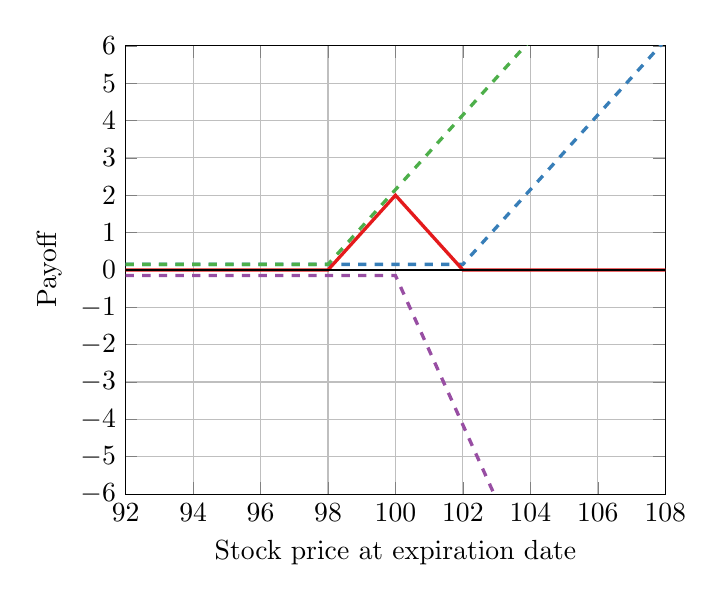
\begin{tikzpicture}
		\begin{axis}[
			%axis lines=middle,
			domain=92:108,
			xtick={92,94,...,108},
			ytick={-6,-5,...,6},
			xmin=92, xmax=108,
			ymin=-6, ymax=6,
			%x label style={at={(axis description cs: 0.5, -0.1)}, anchor=north},
			%y label style={at={(axis description cs:-0.1,1)},anchor=south},
			grid = major,
			xlabel={Stock price at expiration date},
			ylabel={Payoff},
			%scaled x ticks=false
		]
		
	\addplot[Set1-B, very thick, dashed] {(\x > 102)*(\x - 102) + 0.15};
  	\addplot[Set1-C, very thick, dashed] {(\x > 98)*(\x - 98) + 0.15};
  	\addplot[Set1-D, very thick, dashed] {2*(\x > 100)*(100 - \x) - 0.15};
 
 	\addplot[Set1-A, very thick] {(\x > 102)*(\x - 102) + (\x > 98)*(\x - 98) + 2*(\x > 100)*(100 - \x)};
 
   \draw[thick, color=black] (axis cs: 60, 0) -- (axis cs: 120, 0);
\end{axis}
\end{tikzpicture}
\end{frame}



\begin{frame}{Butterfly - 3}
\justify
An example: a butterfly at strikes 99, 100 and 101.

\centering
	\begin{tikzpicture}
		\begin{axis}[
			width = \textheight,
			height = \textheight*0.5,
			domain=92:108,
			%axis lines=middle,
			xtick={92,94,...,108},
			ytick={0,...,6},
			xmin=92, xmax=108,
			ymin=-1, ymax=3,
			%x label style={at={(axis description cs: 0.5, -0.1)}, anchor=north},
			%y label style={at={(axis description cs:-0.1,1)},anchor=south},
			grid = major,
			ylabel={Payoff},
			xlabel={Stock price at expiration date},
			%scaled x ticks=false
		]
		
 	\addplot[Set1-A, very thick, samples at={92,92.1,...,108}] {(\x > 99)*(\x - 99) + (\x > 101)*(\x - 101) + 2*(\x > 100)*(100 - \x) + 0.05};
 
   \draw[thick, color=black] (axis cs: 60, 0) -- (axis cs: 120, 0);
\end{axis}
\end{tikzpicture}

\justify
As we reduce the distance between the wings, the butterfly becomes closer to a bet that the underlying asset price will end up around the central strike.
\end{frame}



\begin{frame}{Butterfly - 4}
\justify
USDRUB butterflies at strikes $K-1$, $K$ and $K+1$..

\centering
\begin{tikzpicture}
\begin{axis}[
			width = \textwidth,
			height = \textheight - 2cm,
			%domain=60:84,
			xtick distance=5,
			ytick distance=0.01,
			xmin=70, xmax=120,
			ymin=0, ymax=0.09,
			scaled y ticks = false,
			yticklabel={\pgfmathprintnumber[fixed, fixed zerofill, precision=2]{\tick}},
			grid = major,
			xlabel={Central strike ($K$)},
			ylabel={Butterfly price, RUB}
]

	\addplot[color = Set1-B, mark = none, thick]
	table[
		x=strike,
		y=fly,
		col sep=comma
	]
	{usdrub_fly.csv};
\end{axis}
\end{tikzpicture}

\scriptsize Data: Moscow Exchange.
\end{frame}



\begin{frame}{Implied distribution}
\centering
\begin{tikzpicture}
\begin{axis}[
			width = \textwidth,
			height = \textheight - 2cm,
			xtick distance=5,
			ytick distance=0.01,
			xmin=70, xmax=120,
			ymin=0, ymax=0.09,
			scaled y ticks = false,
			yticklabel={\pgfmathprintnumber[fixed, fixed zerofill, precision=2]{\tick}},
			grid = major,
			xlabel={Strike ($K$)},
			ylabel={Probability density},
			legend entries = {
				\small Implied,
				\small Log-normal
			},
  			legend cell align={left},
 		 	legend style={at={(0.97,0.97)},anchor=north east}
]

	\addplot[color = Set1-B, mark = none, thick]
	table[
		x=strike,
		y=implied_density,
		col sep=comma
	]
	{usdrub_implied_density.csv};
	
	\addplot[color = Set1-A, mark = none, dashed, thick]
	table[
		x=strike,
		y=lognormal_density,
		col sep=comma
	]
	{usdrub_implied_density.csv};
\end{axis}
\end{tikzpicture}

\scriptsize Data: Moscow Exchange.
\end{frame}



\begin{frame}{Implied distribution - 2}
\justify
Usually option prices imply a distribution that is different from the log-normal distribution. Quite often we observe fat tails and skewness to the left or to the right.

\justify
There are two probable explanations to this fact:
\begin{itemize}
\item Market participants correctly anticipate higher probability of extreme outcomes.
\item Market participants are so scared of extreme outcomes that they are willing to pay for insurance. Risk-averse investors create additional demand for insurance and pull option premiums higher than the "fundamentally fair"\ level.
\end{itemize}

\justify
As long as we can trade in liquid options to hedge more complex illiquid derivatives, we don't need to know which explanation is correct.
\end{frame}



\begin{frame}{Volatility models}
\justify
The existence of volatility smiles refutes the hypothesis of geometric Brownian motion with constant volatility. How should we change the model so that it explains the smile, i.e. yields the same premiums that we observe in the market?

\justify
\begin{itemize}
\item Local volatility.
\item Stochastic volatility.
\item Stochastic local volatility.
\item Stochastic local volatility with jumps.
\item ...
\end{itemize}
\end{frame}



\begin{frame}{Local volatility}
\justify
Geometric Brownian motion:
\begin{align*}
\frac{dS_t}{S_t} = \mu dt + \sigma\xi\sqrt{dt}, \quad \xi \sim \mathcal{N}(0, 1), \sigma = const
\end{align*}

\justify
Local volatility:
\begin{align*}
\frac{dS_t}{S_t} = \mu dt + \sigma(S_t, t)\xi\sqrt{dt}, \quad \xi \sim \mathcal{N}(0, 1)
\end{align*}

\justify
Volatility $\sigma(S_t, t)$ now depends on the underlying price and on time. For example, suppose that EURUSD will drop dramatically from the current level 1.06 to 0.86. This drop will probably trigger a panic in the market, and the exchange rate will be more volatile than usual.
\end{frame}



\begin{frame}{Stochastic volatility}
\justify
Geometric Brownian motion:
\begin{align*}
\frac{dS_t}{S_t} = \mu dt + \sigma\xi\sqrt{dt}, \quad \xi \sim \mathcal{N}(0, 1), \sigma = const
\end{align*}

\justify
Stochastic Alpha-Beta-Rho (SABR) model:
\begin{align*}
dF_t &= \sigma_t(F_t)^\beta \sqrt{dt}\xi, \quad \xi \sim \mathcal{N}(0, 1) \\
d\sigma_t &= \alpha\sigma_t\sqrt{dt}\psi, \quad \psi \sim \mathcal{N}(0, 1) \\
Cov(\xi, \psi) &= \rho
\end{align*}

\justify
$\alpha$ is volatility of volatility.

$\beta$ is skewness coefficient.

$\rho$ is correlation between volatility and asset price.
\end{frame}



\begin{frame}{Model calibration}
\justify
All volatility models are calibrated or fitted to the market. We tune internal model parameters, such as $\alpha$, $\beta$ and $\rho$ in SABR model. We search for those values that make the model replicate market prices of liquid options. Then we can use this calibrated model to price something that is not observable in the market.

\begin{align*}
&\text{Market prices} \Rightarrow \\
&\text{Internal parameters} \Rightarrow \\
&\text{Premiums for arbitrary exotic and illiquid options}
\end{align*}

\justify
Market prices of liquid vanilla options are part of the observed reality. Models and parameters are our assumptions. We use these assumptions to price exotic or illiquid derivatives.
\end{frame}



\begin{frame}{Bonus: variance swap}
\justify
A \alert{variance swap} is a financial derivative whose payoff depends on realized variance of an underlying asset during a specified period. It allows betting on (or hedging against) future volatility.

\justify
Consider a variance swap at strike $\sigma_K^2$ (volatility squared). Notional amount is $N$ dollars, and reference period contains $n$ trading days. The buyer's payoff at maturity is then
\begin{align*}
P = N(\sigma_R^2 - \sigma_K^2)
\end{align*}

where $\sigma_R^2$ is realized daily variance of the underlying asset,
\begin{align*}
\sigma_R^2 = \frac{252}{n-1}\sum\limits_{i=1}^{n}\left(\ln\frac{S_i}{S_{i-1}}\right)^2
\end{align*}
\end{frame}



\begin{frame}{Bonus: pricing a variance swap}
\justify
Fun fact: it is possible to replicate a variance swap of maturity $T$ with a portfolio of vanilla calls and puts of the same maturity. Each vanilla option in the replicating portfolio has a weight of $1/K^2$.

\begin{align*}
\sigma^2_K &= \frac{2e^{rT}}{T}\left(
\int\limits_{0}^{F}\frac{P(K)}{K^2}dK + 
\int\limits_{F}^{\infty}\frac{C(K)}{K^2}dK
\right) \\
F &= Se^{rT}
\end{align*}

\justify
This formula does not depend on Black-Scholes assumptions, it is model-independent. We can derive fair strike of a variance swap (market expectation of future variance) from market premiums for vanilla calls and puts.
\end{frame}



\begin{frame}{Bonus: VIX index}
\justify
The Chicago Board Options Exchange Volatility Index (\alert{VIX}) measures volatility of 30-days S\&P\,500 options. This is not Black-Scholes implied volatility (which would depend on an option strike). The index is derived as a price of a variance swap from all liquid vanilla options (i.e. across a range of strikes).

\justify
VIX is often referred to as "fear gauge" in the press. When investors are nervous, they rush to buy insurance, bid option prices higher, and hence increase the VIX.

\justify
VIX has a twin named RVOL, which measures realized volatility.
\end{frame}



\begin{frame}{Bonus: VIX and realized volatility}
\centering
\begin{tikzpicture}
\begin{axis}[
  width=\textwidth,
  height=\textheight - 1cm,
  date coordinates in=x,
  date ZERO=2012-01-01,
  xtick={2002-01-01, 2005-01-01, 2010-01-01, 2015-01-01, 2020-01-01},
  minor xtick={2003-01-01, 2004-01-01, 2006-01-01, 2007-01-01, 2008-01-01, 2009-01-01, 2011-01-01, 2012-01-01, 2013-01-01, 2014-01-01, 2016-01-01, 2017-01-01, 2018-01-01, 2019-01-01, 2021-01-01, 2022-01-01, 2023-01-01},
  ytick={10, 20, ..., 100},
%  minor ytick={-0.75, -0.25, 0.25, 0.75, 1.25},
  xticklabel={\year},
  xmin=2002-01-01,
  xmax=2024-01-01,
  ymin=0,  ymax=100,
  grid=both,
  yticklabel={\pgfmathprintnumber{\tick}\%},
  xlabel near ticks,
  ylabel near ticks,
legend entries = {
				\small VIX,
				\small RVOL
			},
  			legend cell align={left},
			legend pos=north west
]

\addplot[color = Set1-A, mark = none,  thick]
	table[
		x=date,
		y=vix,
		col sep=comma
	]
	{vix_and_rvol.csv};

\addplot[color = Set1-B, mark = none, dotted, very thick]
	table[
		x=date,
		y=rvol,
		col sep=comma
	]
	{vix_and_rvol.csv};
\end{axis}
\end{tikzpicture}
\small Data: CBOE
\end{frame}



\begin{frame}{Bonus: how deep is the rabbit hole?}
\justify
1. There is the U.S. stock market.

\justify
2. There is S\&P\,500 stock market index.

\justify
3. There are S\&P\,500 futures and options.

\justify
4. There is VIX index to measure volatility of  S\&P\,500 options.

\justify
5. There are VIX futures and options. Underlying asset of a VIX option is volatility of S\&P\,500 options.
\end{frame}


\end{document}

